\section{Indexing Workflows}
\label{sec:indexation}

This section shows how workflows have been indexed using a generalized trie structure\footnote{Trie comes from the word re{\bf Trie}val indicating the process of information accessing but it is also called suffix tree.} and a serialization process. Workflows are a common way of providing and preserving scientific methods by explicitly encoding their processes. They are defined as directed acyclic graphs (DAG) and in Wf4Ever have been described by using both wfdesc and wfprov vocabularies. Therefore, a workflow $wf$ can be defined as a set of $Processes_{wf}$ and $Params_{wf} \quad | \quad wf = Processes_{wf} \cup Params_{wf}$ where the $Processes_{wf}$ are the definition of specific tasks to be executed, and $Params_{wf}$ defines the inputs and outputs of those tasks. On the other hand, a trie structure is an ordered tree data structure that allows to store dynamically a vector or an associative array where the keys are the values being stored itself. The main characteristic of this structure is absence of tree nodes being used for storing the key associated with that node but the position of the node within the tree defines the key. Another characteristic of this structure is that all the descendants of a node have a common prefix and therefore allows indexing simultaneously complete or partial paths to a specific node. \\

For our purposes of indexing a workflow, or generally speaking any DAG, by using a trie structure as a sequence of items which represents the DAG partially or completely for later accessing, a preprocessing of the set of workflows is needed as a first step. For accomplishing with this preprocessing goal of adapting a DAG to the trie indexing structure we have used one of the possible topological orders of a DAG. It is known that any DAG has at least one topological ordering which assures that if a vertex $u$ is linked through an edge to vertex $v$, then after sorting it the vertex $u$ will come before $v$ in ordering. This topological ordering does not have to be unique and therefore a DAG could be defined by multiple topological sorts. Similarly to~\cite{Matono03anindexing}, in order to avoid the possibility of having similar workflows defined in  different ways within the same indexing structure, we have chosen the lexicographical order of processes as common criteria to be applied. Therefore, the chosen overall used criteria for ordering the DAG sequentially has been both the topological and lexicographical orders. \\

The figure~\ref{fig:sorting-workflow} shows how the "Extract proteins using a gi - output as fasta file"~\footnote{http://www.myexperiment.org/workflows/1182.html} example which was obtained from ProvBench data set~\cite{khalid_13}, is sorted by applying our criteria. One of the main advantages of this approach is that after transforming the DAG workflow into a sequential linked set of resources it can be indexed almost instantaneously and the time for searching and exact matching is linear with the size of the tree which is also directly related to the vocabulary size of the domain.

\begin{figure*}[ht!]
\centering
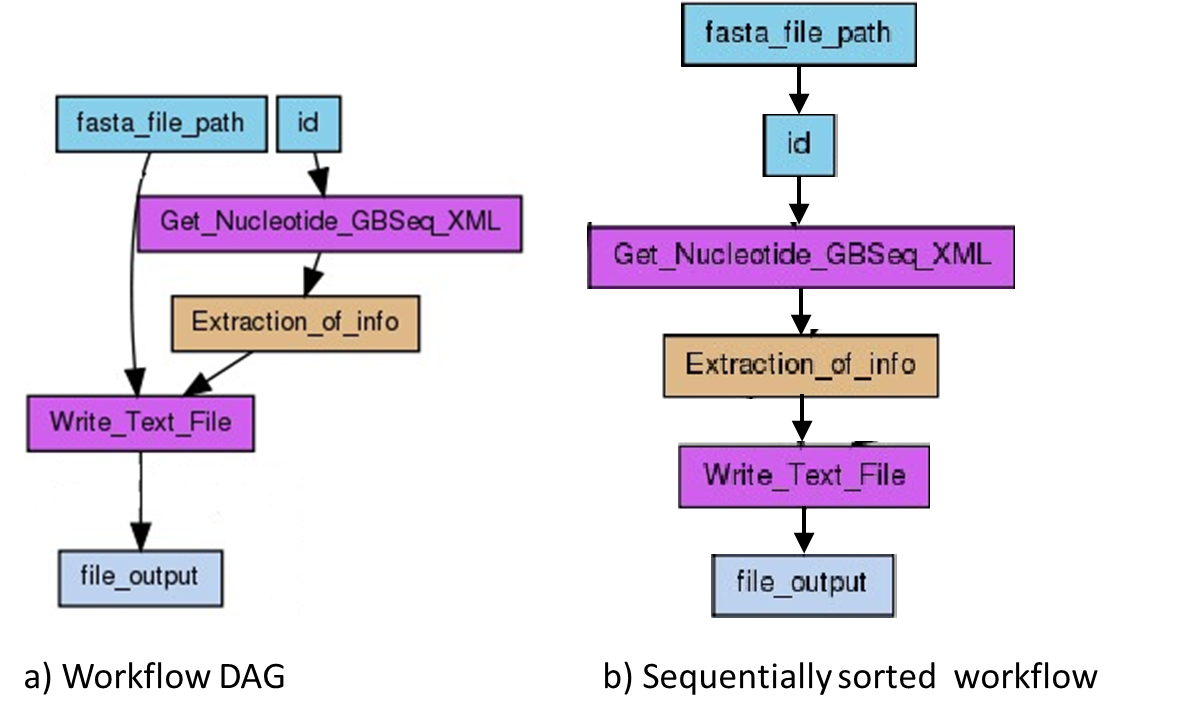
\includegraphics[scale=0.70]{Figures/sorting-workflow.png}
\caption{\textcolor{black}{Sorting the "Extract proteins using a gi - output as fasta file" example obtained from ProvBench}}
\label{fig:sorting-workflow}
\end{figure*}

\subsection{Applications and Implementation}
In order to provide scientists with searching and design capabilities we have implemented two different web services which makes use of the above introduced indexing structure for accessing to workflows and recommend next steps given the previous ones. It is worth highlighting that the implemented indexing structure could be also used for other purposes as the discovery of frequent patterns by using the collected statistical information and mining the semantic trie structure which would take full advantage of the intrinsic sequential ordering of the trie structure. 

The implementation of both services (searching and next step recommendation) has been done applying the guidelines of the Wf4Ever project. Both services are REST and can be called by an HTTP GET method which upon on ACCEPT headers may return XML or JSON formats. Also for implementation purposes we have encapsulated the trie indexing structured in order to provided the above presented services.
 
\subsubsection{Searching}

This service~\url{http://sandbox.wf4ever-project.org/wfabstraction/rest/search} searches for those workflows which contain a specific sequence of processes providing on real time a list including all of them. The service accepts an array of processes' names as input parameter process[] (e.g. process?=p1\&p2\&p3). Therefore the general call would be of the form:~\url{http://sandbox.wf4ever-project.org/wfabstraction/rest/search{?process[]}}.\\

The output is an XML or JSON structure with the following attributes: 
\begin{itemize}
\item \textbf{Process\_id}: is the name of the process or processes used in the query.
\item \textbf{freq}: is the number of times that the sequence of processes appears in other workflows.
\item \textbf{URIs}: are the URIs of the workflows where the sequence appears. 
\end{itemize}

\subsubsection{Next step recommendation}
The proposed trie structure captures the provenance of workflows execution associated to scientific experiments allowing
their indexation based on the temporal information that they contain. The trie structure is also updated to gather
the needed statistics for mining the execution of workflows and provide the recommended next process based on how frequent 
a pattern of use occurs. So far we collected the number of times a process occurs in the dataset and also the probability associated 
to that pattern given the set of patterns of the same size. The fact that the exact matching searching is linear with the size of the tree (which is dependent of the use vocabulary, in our case the domain has been restricted to the set of processes included in ProvBench~\cite{khalid_13}) makes it very suitable for 
this type of applications. The implemented service~\url{http://sandbox.wf4ever-project.org/wfabstraction/rest/recommend} accepts an array of processes' names as input parameter process[] (e.g. process?=p1\&p2\&p3) and its general call would be of the form:~\url{http://sandbox.wf4ever-project.org/wfabstraction/rest/recommend{?process[]}} \\

The output is an XML or JSON structure with different attributes:
\begin{itemize}
\item \textbf{Id}: is the name of the recommended process for that input query.
\item \textbf{freq}:  is the number of times that it appears in different workflows.
\item \textbf{prob}:  is the probability of the given recommendation taking into account the whole set of possible next steps.
\end{itemize}